\let\negmedspace\undefined
\let\negthickspace\undefined
\documentclass[journal,12pt,twocolumn]{IEEEtran}
\usepackage{cite}
\usepackage{amsmath,amssymb,amsfonts,amsthm}
\usepackage{algorithm}
\usepackage{graphicx}
\usepackage{textcomp}
\usepackage{xcolor}
\usepackage{txfonts}
\usepackage{listings}
\usepackage{enumitem}
\usepackage{mathtools}
\usepackage{gensymb}
\usepackage{comment}
\usepackage[breaklinks=true]{hyperref}
\usepackage{tkz-euclide}
\usepackage{listings}
\usepackage{gvv}
\def\inputGnumericTable{}
\usepackage[latin1]{inputenc}
\usepackage{color}
\usepackage{array}
\usepackage{longtable}
\usepackage{calc}
\usepackage{multirow}
\usepackage{hhline}
\usepackage{ifthen}
\usepackage{lscape}

\newtheorem{theorem}{Theorem}[section]
\newtheorem{problem}{Problem}
\newtheorem{proposition}{Proposition}[section]
\newtheorem{lemma}{Lemma}[section]
\newtheorem{corollary}[theorem]{Corollary}
\newtheorem{example}{Example}[section]
\newtheorem{definition}[problem]{Definition}
\newcommand{\BEQA}{\begin{eqnarray}}
\newcommand{\EEQA}{\end{eqnarray}}
\newcommand{\define}{\stackrel{\triangle}{=}}
\theoremstyle{remark}
\newtheorem{rem}{Remark}
\begin{document}

\bibliographystyle{IEEEtran}
\vspace{3cm}

\title{NCERT Discrete - 11.9.1.8}
\author{EE23BTECH11045 - Palavelli Srija$^{*}$% <-this % stops a space
}
\maketitle
\newpage
\bigskip

\renewcommand{\thefigure}{\theenumi}
\renewcommand{\thetable}{\theenumi}

\vspace{3cm}
\textbf{Question 11.9.1.8:} 
\begin{enumerate}
\item Find the seventh term of the sequence where the nth term is given by $a_n= \frac {n^2}{2^{n}}$

\end{enumerate}
\textbf{Solution: }
\begin{align}
 x(n) &= \frac{(n+1)^2}{2^{(n+1)}}u(n)
\end{align}
\begin{table}[h!]
    \centering
    \begin{tabular}{|c|c|c|}
    \hline
     \textbf{Symbol} & \textbf{Value} \\
    \hline
     $x_1(n)$ & $\left\{5,55,555...\right\}$ \\[6pt]
    \hline
     $x_2(n)$ & $\left\{0.6,0.66,0.666...\right\}$ \\[6pt]
   
     
    \hline
\end{tabular}

    \caption{Input Parameters}
    \label{tab:table_9.8.1}
   \end{table}
\begin{align}
x(6) &= \frac{(6+1)^2}{2^{(6+1)}}\\
x(6) &= \frac {49}{128}
\end{align}
The Z transform of x(n) is given by
\begin{align}
X(z) &= \sum_{n=-\infty}^{\infty} \frac{(n+1)^2}{2^{(n+1)}}u(n) z^{-n}\\
X(z) &= \sum_{n=0}^{\infty} \frac {(n+1)^2}{2^{(n+1)}}z^{-n}
\end{align}
Using differentiation and scaling property
\begin{align}
X(z) &=  \frac {(1+(2z)^{-1})}{2(1-(2z)^{-1})^{3}}; \quad \abs{z} > \frac{1}{2}
\end{align}
\begin{figure}[h!]
    \centering
    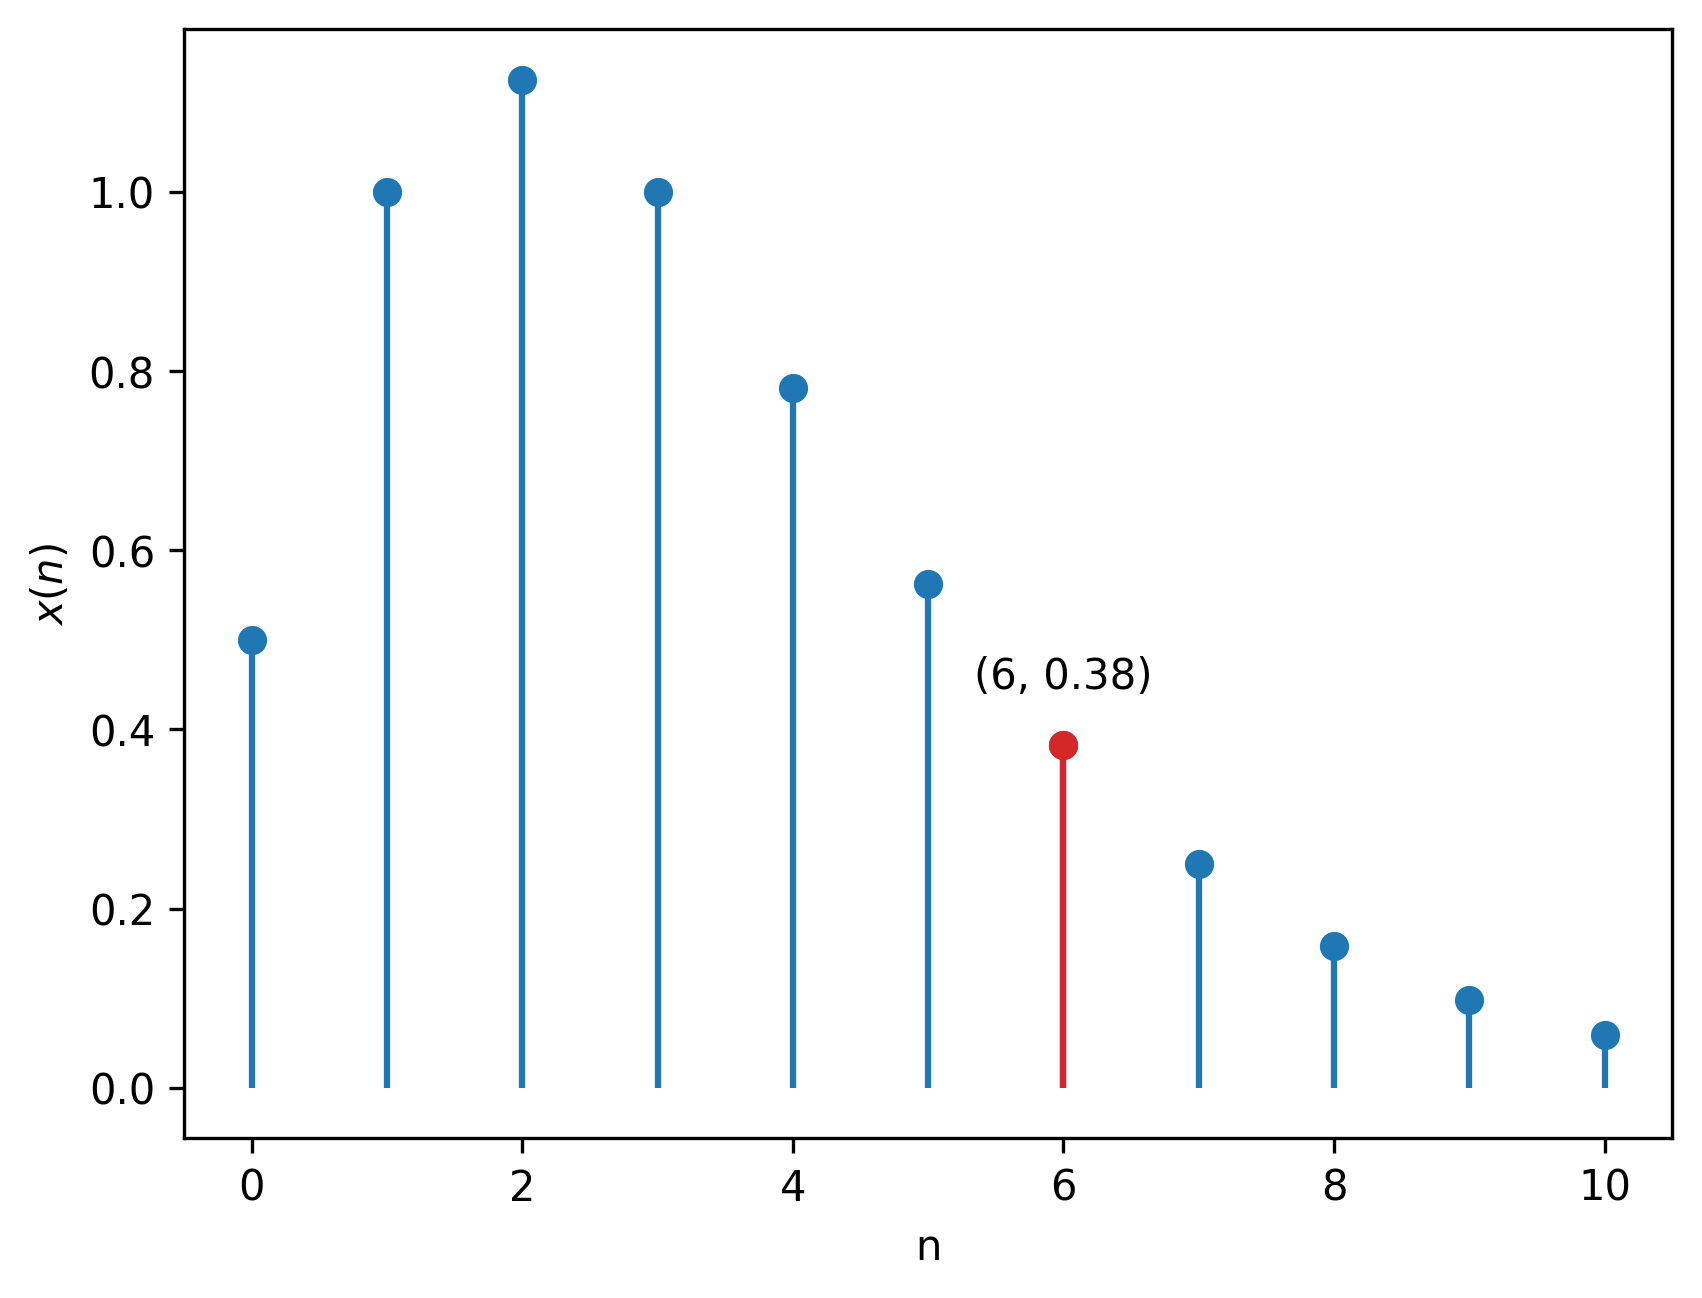
\includegraphics[width=\columnwidth]{figs/plot.png}
    \caption{stem plot of $x(n)$}
    \label{fig:1}
\end{figure}
\end{document}

